% !TEX root = ../main.tex

\section{Background}
\label{section:background}

\mdr{Be very concise here. Introduce notation, terminology. Cut all the side tracks, and set up only the things that are needed to understand the method in the next section. Move discussion of related work to last section but one.}

\subsection{Learning algorithms for SIMPUL problems}
% \textbf{we introduce our sub-problem}

There seems to exist a consensus over the terms \emph{multiclass learning} and
\emph{multilabel learning}. The former denotes a setting where  meaning mutually exclusive and mutually inclusive
labels, respectively~\cite{multilabelMethods}. Multilabel learning can
therefore be seen as a subdomain of multiclass learning, where more than one
class can be correct for the same example. We propose the term single-instance
as opposed to multi-instance learning~\citep[e.g.,][]{multiInstance,
multiInstanceMultiLabel}, for which it is considered natural to first segment
an image, text or sound before performing prediction on each of the segments.

The single/multi instance distinction helps explain why the abstract aspect
can be considered implicit in SIMPUL. Beyond identifying object types (see
YOLO \cite{YOLO} and its successors), performing face recognition (see FaceNet
\cite{FaceNet} and its successors) on segments of an image, neural networks
are increasingly becoming better at predicting more abstact concepts via
deeper networks, representation learning and self-supervision~\citep[see,
e.g.,][]{SS,Rep}. Towards this goal, there is a significant volume of recent
work on building neural networks with a high-level of abstract understanding
in the embedding space~\mdr{REF}. However, research on developing optimization
frameworks that are adapted for these abstract concepts in the output space is
limited.

% \textbf{current state of the art, related work}
The existing optimization frameworks are still largely based on variations of
the cross-entropy loss, with recently some advances in dealing with
sparsity in the output space~\citep[see, e.g.,][]{focalLoss,tencent}. Existing measures for multilabel prediction can be
divided into two fields: the \emph{fit-data-to-algorithm} (a.k.a \emph{problem transformation}) and \emph{fit-algorithm-to-data} (a.k.a \emph{algorithm
adaptation}) approaches~\cite{multilabelReview}. Although it is less in use in the literature, we prefer the first definitions because they are less ambiguous. In the case of fit-data-to-algorithm,
multilabel classification is reframed as a binary, multiclass classification
or label ranking problem. In the case of fit-algorithm-to-data, one tries to
adapt multiclass algorithms to the problem.

\subsubsection{fit-data-to-algorithm} For the purpose of problem transformation,
we define \(\mathcal{L}_{\text {multiclass}}\), a class of loss functions that
minimize predictions in relative terms. Binary cross-entropy, logistic regression and their
variants, such as focal loss or hinge loss are common choices when it comes to
multiclass prediction. Cross-entropy loss can be formulated as
\(\mathcal{L}_{\text {CE}}=-\sum \log \left(p_{i}\right)\). Note that
minimizing binary cross-entropy is equivalent to maximizing for log-likelihood
\cite[Section 4.3.4]{Bishop}. More generally, the \emph{problem
transformation} formulation amounts to minimizing the loss on a class of
neural networks, such that
%
\begin{equation}
\underset{\mathcal{L}_{\text {multiclass}}} {\min} \mathcal{F}\left(\cdot ;
\Theta; \mathcal{L}_{\text {multiclass}} (\mathbf{y}, \hat{\mathbf{y}})
\right),
\end{equation}
%


Astonishingly, state-of-the-art CNN and attention based models for text~\cite{XLNet, bigBird, } and image respectively still use the problem transformation framework even when fine-tuning for multilabel classification tasks on datasets like IMDB, Yelp-2, Yelp-5, DBpedia, AG, Amazon-2, and Amazon-5 for text and .  XLNet uses adversarial loss, BigBird uses cross-entropy as most Bert models do...

\hvk{related work of problem transformation here}

\subsubsection{fit-algorithm-to-data}
In the context of \emph{algorithm
adaptation}, where the number of positive labels in the groundtruth is unknown
a priori \daan{this is not a property of algo adapt per se, right?}, we aim to
both obtain a propensity of each label being true and a prediction of the
number of true labels:
%
\begin{equation}
\underset{\mathcal{L}_{\text {multiclass}}, \mathcal{L}_{\text {count}}}
{\min} \mathcal{F}\left(\cdot ; \Theta; \mathcal{L}_{\text {multiclass}}
(\mathbf{y}, \hat{\mathbf{y}}) + \lambda \mathcal{L}_{\text {count}}
(\mathbf{n}, \hat{\mathbf{n}})\right),
\end{equation}
%
where \(n_i = \sum_j \mathds{1}_{\mathbf{y_i^j} = 1}\) is the count of
positive labels per example. We thus impose a constraint for the retrieval of
label counts. For example, a cross-entropy loss surrogate would penalize for the number of wrongly predicted
labels \(\mathcal{L}_{\text {CE+N}}= \mathcal{L}_{\text {CE}} + \lambda (\sum
tp / \sum p)\), with \(t p=\sum_{i \in Y^{+}} \mathds{1}_{\mathbf{p_i} \geq
b}\) and \(b\) a threshold to be defined. With its multitask framework
(predict label prediction propensity and label count) \cite{multitaskLabel}
corresponds to that type of infrastructure. \todo{tencent loss}. The latter
formulation is most straightfoward but suffers from higher parametrization and
the lack of modelling of the interactions between label counts and label
prediction.

Early representatives of algorithm adaptation stem from heterogenous
domains of machine learning. Multi-Label k-Nearest Neighbors \cite{ML-KNN},
Multi-Label Decision Tree \cite{ML-DT}, Ranking Support Vector Machine
\cite{multilabelSVM} and Backpropagation for Multi-Label Learning
\cite{multilabelBackprop}. More recently, two papers introduced the idea of
multitask learning for \emph{label prediction} and \emph{label count
prediction} for text (ML\(_{\text{NET}}\)) \cite{multitaskLabel} and image
\cite{multitaskLabelImages} data. The latter research is loosely catered
towards object detection (although not formally presented as such) and is thus
out-of-scope: elements in a picture are predicted that tend to be unilabel as
defined by the groundtruth (e.g. cat, flower, vase, person, bottle etc.).

\subsubsection{design-algorithm-for-data}

To mitigate these issues, we propose a unified loss formulation,
namely
%
\begin{equation}
\underset{\mathcal{L}_{\text {multilabel}}} {\min} \mathcal{F}\left(\cdot ;
\Theta; \mathcal{L}_{\text {multilabel}} (\mathbf{y}, \hat{\mathbf{y}},
\mathbf{n}, \hat{\mathbf{n}}) \right),
\end{equation}
%
Although predictions and counts explicitly appear in that formulation,
\(\mathcal{L}_{\text {multilabel}}\) can optimize for both metrics implicitly
(see proposed \emph{sigmoidF1} below).

\todo{further justify our approach here}

\subsection{Towards smooth loss functions that optimize learning
in SIMPUL problems}
In summary, in the case of \emph{problem transformation},
cross-entropy losses are used at training time and thresholding is done at
inference time. In the case of \emph{algorithm adaptation}, elements of the
learning algorithm are changed (such as the backpropagation procedure or the
tasks). We propose a solution aligned with the algorithm adaptation paradigm,
where we propose a custom loss formulation to solve SIMPUL problems.

In machine learning prediction tasks, the probabilistic measure (or a reversible
transformation of a probabilistic measure such as a sigmoid or a softmax
function) are compared to binary values in the case of binary encoding of
classes. At inference time, if the number $n_i$ of labels to be predicted per
example is known a priori, it is natural to assign the $top_{n_i}$ predictions
to that example~\cite{lossTopKError, topKmulticlassSVM}. If the number of
labels per example is unknown a priori, the question remains at inference time
as to how to extract information about the number of labels to assign to each
example, aside from the propensity of labels to be assigned. This is generally
done via a \emph{decision threshold}, that can be set globally for all
examples. This threshold can optimize for specificity or
sensitivity~\cite{decisionThreshold}. We propose a method where this threshold
is implicitely defined, thanks to the use of metrics that already penalize for
wrong label counts.

Thresholding accross classes or examples can be an issue as soon as the number of labels to predict is unknown. Certain variants of cross-entropy loss accommodate imbalanced label data  \cite{focalLoss}, but remain agnostic towards the number of labels to predict. Solutions have been tailored to that end, starting with determining an ideal global \emph{threshold} depending on use-cases \cite{threshForF1}, or per-class-thresholding after training \cite{moviePosters} and eventually abstracting the threshold away via a \emph{soft-F1} measure \cite{softF1}. In the latter two cases, the task is to predict genre from movie posters.

The proposed method is positioned in the lineage of \emph{algorithm adaptation}, using \emph{metric as losses} and allowing for dynamic \emph{thresholding}. 

\begin{figure}[htbp]
\centering
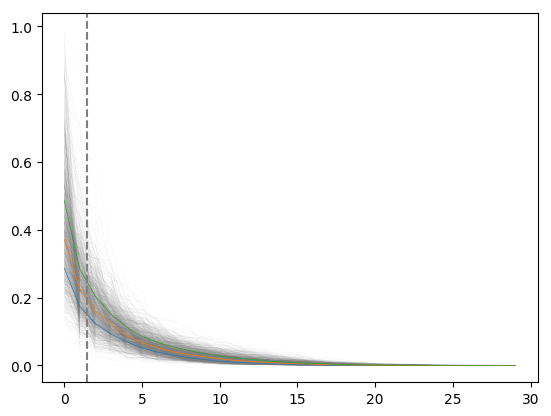
\includegraphics[width=.9\linewidth]{./images/knee.png}
\caption{\label{fig:knee}
\todo{nicer plot on another dataset (this is from RTL)}
Ordered per-label cross-entropy predictions for each example (each grey line) with the median (orange) and IQR (green \& blue) over all examples. Determining a global threshold can be related to visually finding the ``knee'' in that median curve (dotted line).}
\end{figure}

\todo{combine the two next paragraphs}

Often, machine learning post-training evaluation metrics (e.g. AUROC, F1) are
not differentiable. There are motivations \todo{which motivations} for
optimizing a model directly on a metric at training time. A general framework
for AUC, AUROC and F1 is presented in \cite{optimizableLosses}, but the
proposed F1 surrogate remains short of being explicitly derived for stochastic
gradient descent. Recently, a similar work has been proposed to train a
Convolutional Neural Network (CNN) from scratch with a few millions of images
and hundreds of labels specifically for multilabel tasks \cite{tencent}. This
task is loosely related to object detection, similarly to
\cite{multitaskLabelImages} mentioned in the previous paragraph.

% \begin{figure}[t]
% \centering
% 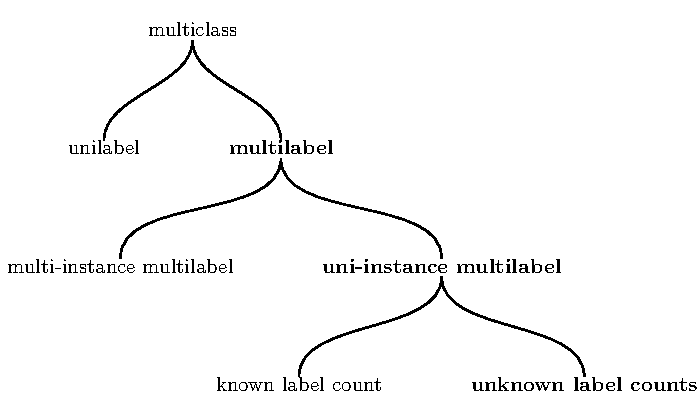
\includegraphics[width=.9\linewidth]{./tree/Tree.pdf}
% \caption{\label{fig:tree} SIMPUL (bold) within the \emph{multiclass}
% nomenclature
% \hvk{figure is not referenced in text, bold is unclear in figure}
% \daan{I think it should go. And if it stays: uni -> single.}
% % Clarifying ``multiclass'' classification problems. In this paper we focus on
% % the uni-instance, multilabel, multiclass classification problem with a
% % varying number of labels (the bottom right hand side of the tree).
% }
% \end{figure}% \mdr{Image source ...}

In a number of retrieval tasks, a model's out of sample accuracy is measured
on metrics such as AUROC, F1 score, etc. These reflect an objective catered
towards evaluating the model over an entire ranking. Due to the lack of
differentiability, these metrics cannot be directly used as loss functions at
training time (in-sample). A seminal study~\cite{optimizableLosses} derived a
general framework for deriving decomposable surrogates to some of these
metrics. We propose our own decomposable F1 surrogate tailored for the problem
at hand.
